\documentclass[12pt]{article}
\usepackage[a4paper, total={7in, 10.5in}, headheight=16pt, headsep=1cm]{geometry}
\usepackage[utf8]{inputenc}
\setcounter{tocdepth}{4}
\setcounter{secnumdepth}{4}
\usepackage[MeX]{polski}
\usepackage[T1]{fontenc}
\usepackage{colortbl}
\usepackage{graphicx}
\usepackage{svg}
\usepackage{upgreek}
\usepackage{amsmath}
\usepackage{caption}
\usepackage{titlesec}
\usepackage{amssymb}
\usepackage{hyperref}
\usepackage{gensymb}
\usepackage{listings}
\usepackage{xcolor}
\usepackage{multirow}
\usepackage{pdfpages}
\usepackage{url}
\usepackage{subfig}
\usepackage{float}
\usepackage{listings}
\usepackage{fancyhdr}
\usepackage{multicol}
\usepackage{float}
\usepackage{adjustbox}
\usepackage[nottoc,numbib]{tocbibind}
\usepackage[scaled=0.8]{beramono} % Smaller font for listings

\renewcommand{\lstlistlistingname}{Spis listingów}

% USTAWIENIA DO SPISU TREŚĆI (HIPERŁĄCZA)

\hypersetup{
     colorlinks=true,
     linkcolor=black,
     filecolor=magenta,      
     urlcolor=black,
     pdfpagemode=FullScreen,
}
\urlstyle{same}

% USTAWIENIA DO KOLORÓW TABEL

\definecolor{green}{RGB}{147, 196, 125}
\definecolor{light_green}{RGB}{182, 215, 168}
\definecolor{red}{RGB}{255, 0, 0}
\definecolor{light_red}{RGB}{255, 101, 101}

%New colors defined below
\definecolor{codegreen}{rgb}{0,0.6,0}
\definecolor{codegray}{rgb}{0.5,0.5,0.5}
\definecolor{codepurple}{rgb}{0.58,0,0.82}
\definecolor{backcolour}{rgb}{0.95,0.95,0.92}

%Code listing style named "mystyle"
\lstdefinestyle{mystyle}{
  commentstyle=\color{codegreen},
  keywordstyle=\color{magenta},
  numberstyle=\tiny\color{codegray},
  stringstyle=\color{codepurple},
  basicstyle=\ttfamily,
  breakatwhitespace=false,         
  breaklines=true,            
  captionpos=t,                    
  keepspaces=true,                 
  numbers=left,                    
  numbersep=5pt,                  
  showspaces=false,          
  showstringspaces=false,
  showtabs=false,                  
  tabsize=2,
  escapechar={|}
  moredelim=**[is][\color{red}]{@}{@},
}

\lstdefinelanguage{JavaScript}{
  morekeywords=[1]{break, continue, delete, else, for, function, if, in,
    new, return, this, typeof, var, void, while, with},
  % Literals, primitive types, and reference types.
  morekeywords=[2]{false, null, true, boolean, number, undefined,
    Array, Boolean, Date, Math, Number, String, Object},
  % Built-ins.
  morekeywords=[3]{eval, parseInt, parseFloat, escape, unescape},
  sensitive,
  morecomment=[s]{/*}{*/},
  morecomment=[l]//,
  morecomment=[s]{/**}{*/}, % JavaDoc style comments
  morestring=[b]',
  morestring=[b]"
}[keywords, comments, strings]

\lstset{
extendedchars=\true,
inputencoding=utf8x
}

\lstset{language=SQL,style=mystyle}

\renewcommand{\lstlistingname}{Kod}

\newfloat{Diagram}{htbp}{grf}

% TYTUŁ I AUTORZY

\begin{document}

\pagestyle{fancy}
\fancyhead{} % clear all header fields
\fancyhead[RO]{\textbf{Integracja systemów informatycznych - projekt}}      % Title
\lhead{
\includegraphics[width=4cm]{pwr_poziom.png}}
\fancyfoot{}
\fancyfoot[C]{\thepage}

\begin{titlepage}
\newcommand{\HRule}{\rule{\linewidth}{0.5mm}} % Defines a new command for the horizontal lines, change thickness here
\center % Center everything on the page
%	LOGO SECTION
\begin{figure}[h]
    \centering
    
\includegraphics[scale=0.21]{pwr-logo.png} \hspace{1cm}
     \raisebox{0.75cm}{
\includegraphics[scale=0.5]{W4N.png}} \hspace{1cm}
\end{figure}
%	HEADING SECTIONSImages
\textsc{\Large Integracja systemów informatycznych}\\[0.5cm] 
\textsc{\large Wtorek 15:15}\\[0.5cm]
%	TITLE SECTION
\HRule \\[0.8cm]
{ \huge \bfseries Wstępne założenia projektowe}\\[0.4cm] 
% 
\HRule \\[0.8cm]
%	AUTHORS SECTION
\begin{minipage}{0.45\textwidth}
\begin{flushleft} \large
\emph{Autorzy:}\\
Marcin \textsc{Goliasz} 273 185\\
Andrzej \textsc{Manderla} 294 692\\
Mateusz \textsc{Gawłowski} 264 463 \\
Wojciech \textsc{Tobolski} 259 357 \\

\end{flushleft}
\end{minipage}
~
\begin{minipage}{0.45\textwidth}
\begin{flushright} \large

\end{flushright}
\end{minipage}\\[5cm]
\end{titlepage}
\newgeometry{bmargin=2cm, tmargin=2cm, lmargin=2cm, rmargin=2cm}
\newpage


\thispagestyle{empty}
\tableofcontents
\newpage
\thispagestyle{empty}

\newpage

\pagenumbering{arabic}

% document sections

\section{Opis projektu i jego celu}
Celem projektu jest zaprojektowanie oraz implementacja rozproszonego systemu informatycznego służącego do kompleksowej obsługi i rejestracji usług medycznych (np. wizyt u lekarza specjalisty). System ma za zadanie cyfryzację procesu umawiania wizyt, automatyzację rozliczeń finansowych oraz usprawnienie komunikacji na linii placówka-pacjent.

\section{Główne funkcjonalności systemu}
\begin{itemize}
    \item \textbf{Rejestracja pacjentów na wizyty:} Wyszukiwanie wolnych terminów, wybór specjalisty oraz rezerwacja wybranego okna czasowego.
    \item \textbf{Zarządzanie kalendarzem wizyt:} Definiowanie dostępności przez lekarzy, blokowanie terminów, odwoływanie wizyt.
    \item \textbf{Obsługa płatności online:} Integracja z bramką płatniczą w celu przedpłaty za zarezerwowaną usługę.
    \item \textbf{Powiadomienia o wizytach:} Automatyczna wysyłka potwierdzeń, przypomnień o zbliżającym się terminie oraz informacji o zmianach statusu (e-mail/kalendarz).
    \item \textbf{Zarządzanie historią wizyt:} Dostęp do archiwum odbytych konsultacji, zaleceń i wystawionych dokumentów.
\end{itemize}

\section{Role użytkowników i ich uprawnienia}
\begin{itemize}
    \item \textbf{Pacjent:}
    \begin{itemize}
        \item Wyszukiwanie terminów i specjalistów.
        \item Rezerwacja, opłacanie i anulowanie własnych wizyt.
        \item Wgląd w historię leczenia i pobieranie rachunków/faktur.
    \end{itemize}
    \item \textbf{Lekarz:}
    \begin{itemize}
        \item Zarządzanie własnym grafikiem i dostępnością.
        \item Przegląd zaplanowanych wizyt na dany dzień/tydzień.
        \item Dodawanie notatek z przebiegu wizyty oraz zaleceń pooperacyjnych/terapeutycznych.
    \end{itemize}
    \item \textbf{Administrator:}
    \begin{itemize}
        \item Zarządzanie kontami użytkowników (personelu i pacjentów).
        \item Konfiguracja usług, cenników oraz systemowych parametrów integracji.
        \item Wgląd w logi systemowe i raporty finansowe.
    \end{itemize}
\end{itemize}

\section{Architektura systemu}
\subsection{Opis systemu rozproszonego}
Architektura opiera się na wzorcu mikroserwisów, co zapewnia niezależne skalowanie, wdrażanie oraz izolację błędów. Komponenty systemu komunikują się ze sobą synchronicznie (REST API) w przypadku operacji wymagających natychmiastowego potwierdzenia, oraz asynchronicznie (RabbitMQ) dla procesów w tle.

\section{Integracje z systemami zewnętrznymi}
\begin{itemize}
    \item \textbf{PayU:} Wykorzystywane do obsługi płatności za wizyty. \texttt{Payment-Service} komunikuje się z API PayU w celu wygenerowania linku do płatności (OrderCreateRequest) oraz nasłuchuje na webhooki (notyfikacje IPN) o zmianie statusu transakcji (np. z \texttt{PENDING} na \texttt{COMPLETED}).
    \item \textbf{Gmail API / Google Calendar API:} \texttt{Notification-Service} wykorzystuje te API do automatycznego dodawania wydarzeń bezpośrednio do kalendarza pacjenta i lekarza oraz wysyłania spersonalizowanych wiadomości e-mail z przypomnieniami.
\end{itemize}

\section{Komunikacja między usługami}
\subsection{REST API i OpenAPI}
Synchroniczna komunikacja (np. pobieranie profilu użytkownika przez \texttt{Appointment-Service}) realizowana jest poprzez bezstanowe API RESTowe. Każdy mikroserwis udostępnia własną dokumentację wygenerowaną zgodnie ze standardem \textbf{OpenAPI 3.0} (dostępną m.in. przez interfejs Swagger UI), co ułatwia kontraktowanie i integrację frontendu z backendem.

\subsection{Walidacja danych (JSON Schema)}
Struktura wszystkich zapytań wejściowych do API (request payloads) jest rygorystycznie walidowana przed przekazaniem do logiki biznesowej z użyciem \textbf{JSON Schema}. Zapobiega to przetwarzaniu niepełnych lub złośliwych danych, odrzucając je na poziomie kontrolera z kodem \texttt{400 Bad Request}.

\subsection{Wykorzystanie RabbitMQ}
RabbitMQ pełni rolę brokera wiadomości dla komunikacji asynchronicznej. Zastosowanie wymiany typu \texttt{Topic} (Topic Exchange) pozwala na elastyczne trasowanie zdarzeń (np. \texttt{appointment.created}, \texttt{payment.success}). Gwarantuje to brak utraty danych w przypadku chwilowej niedostępności usług powiązanych.

\section{Procesy biznesowe (BPMN)}
\begin{figure}[H]
  \centering
  \adjustbox{max width=\textwidth}{
    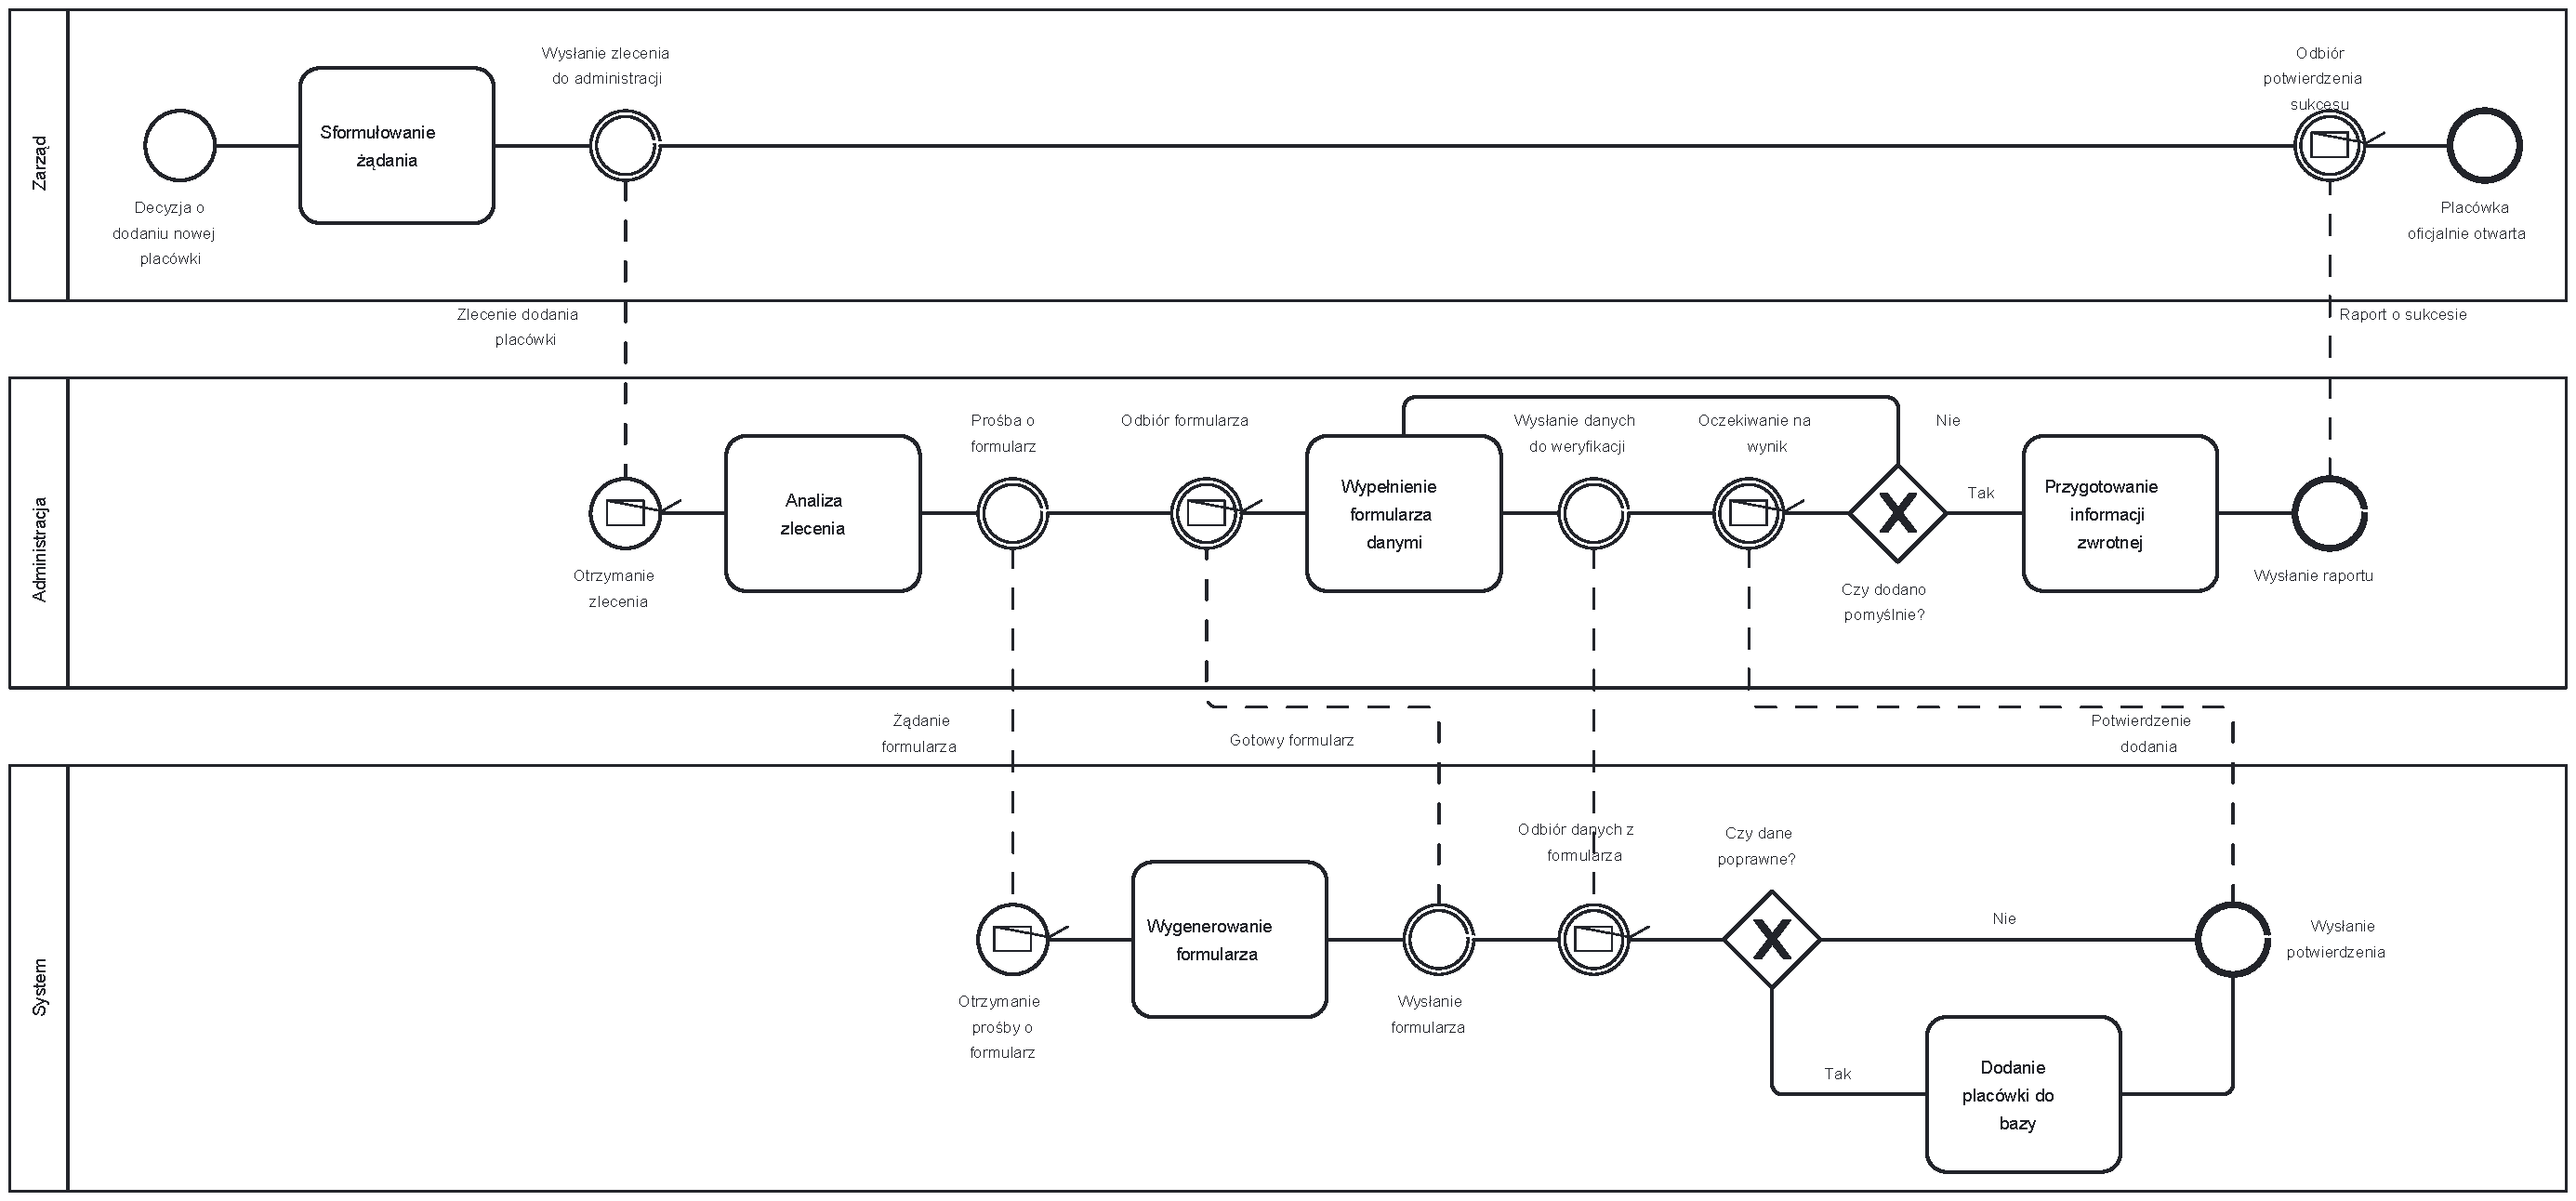
\includegraphics{bpmn/FacilityRegistration.pdf}
  }
  \caption{Rejestracja placówki}
\end{figure}

\begin{figure}[H]
  \centering
  \adjustbox{max width=\textwidth}{
    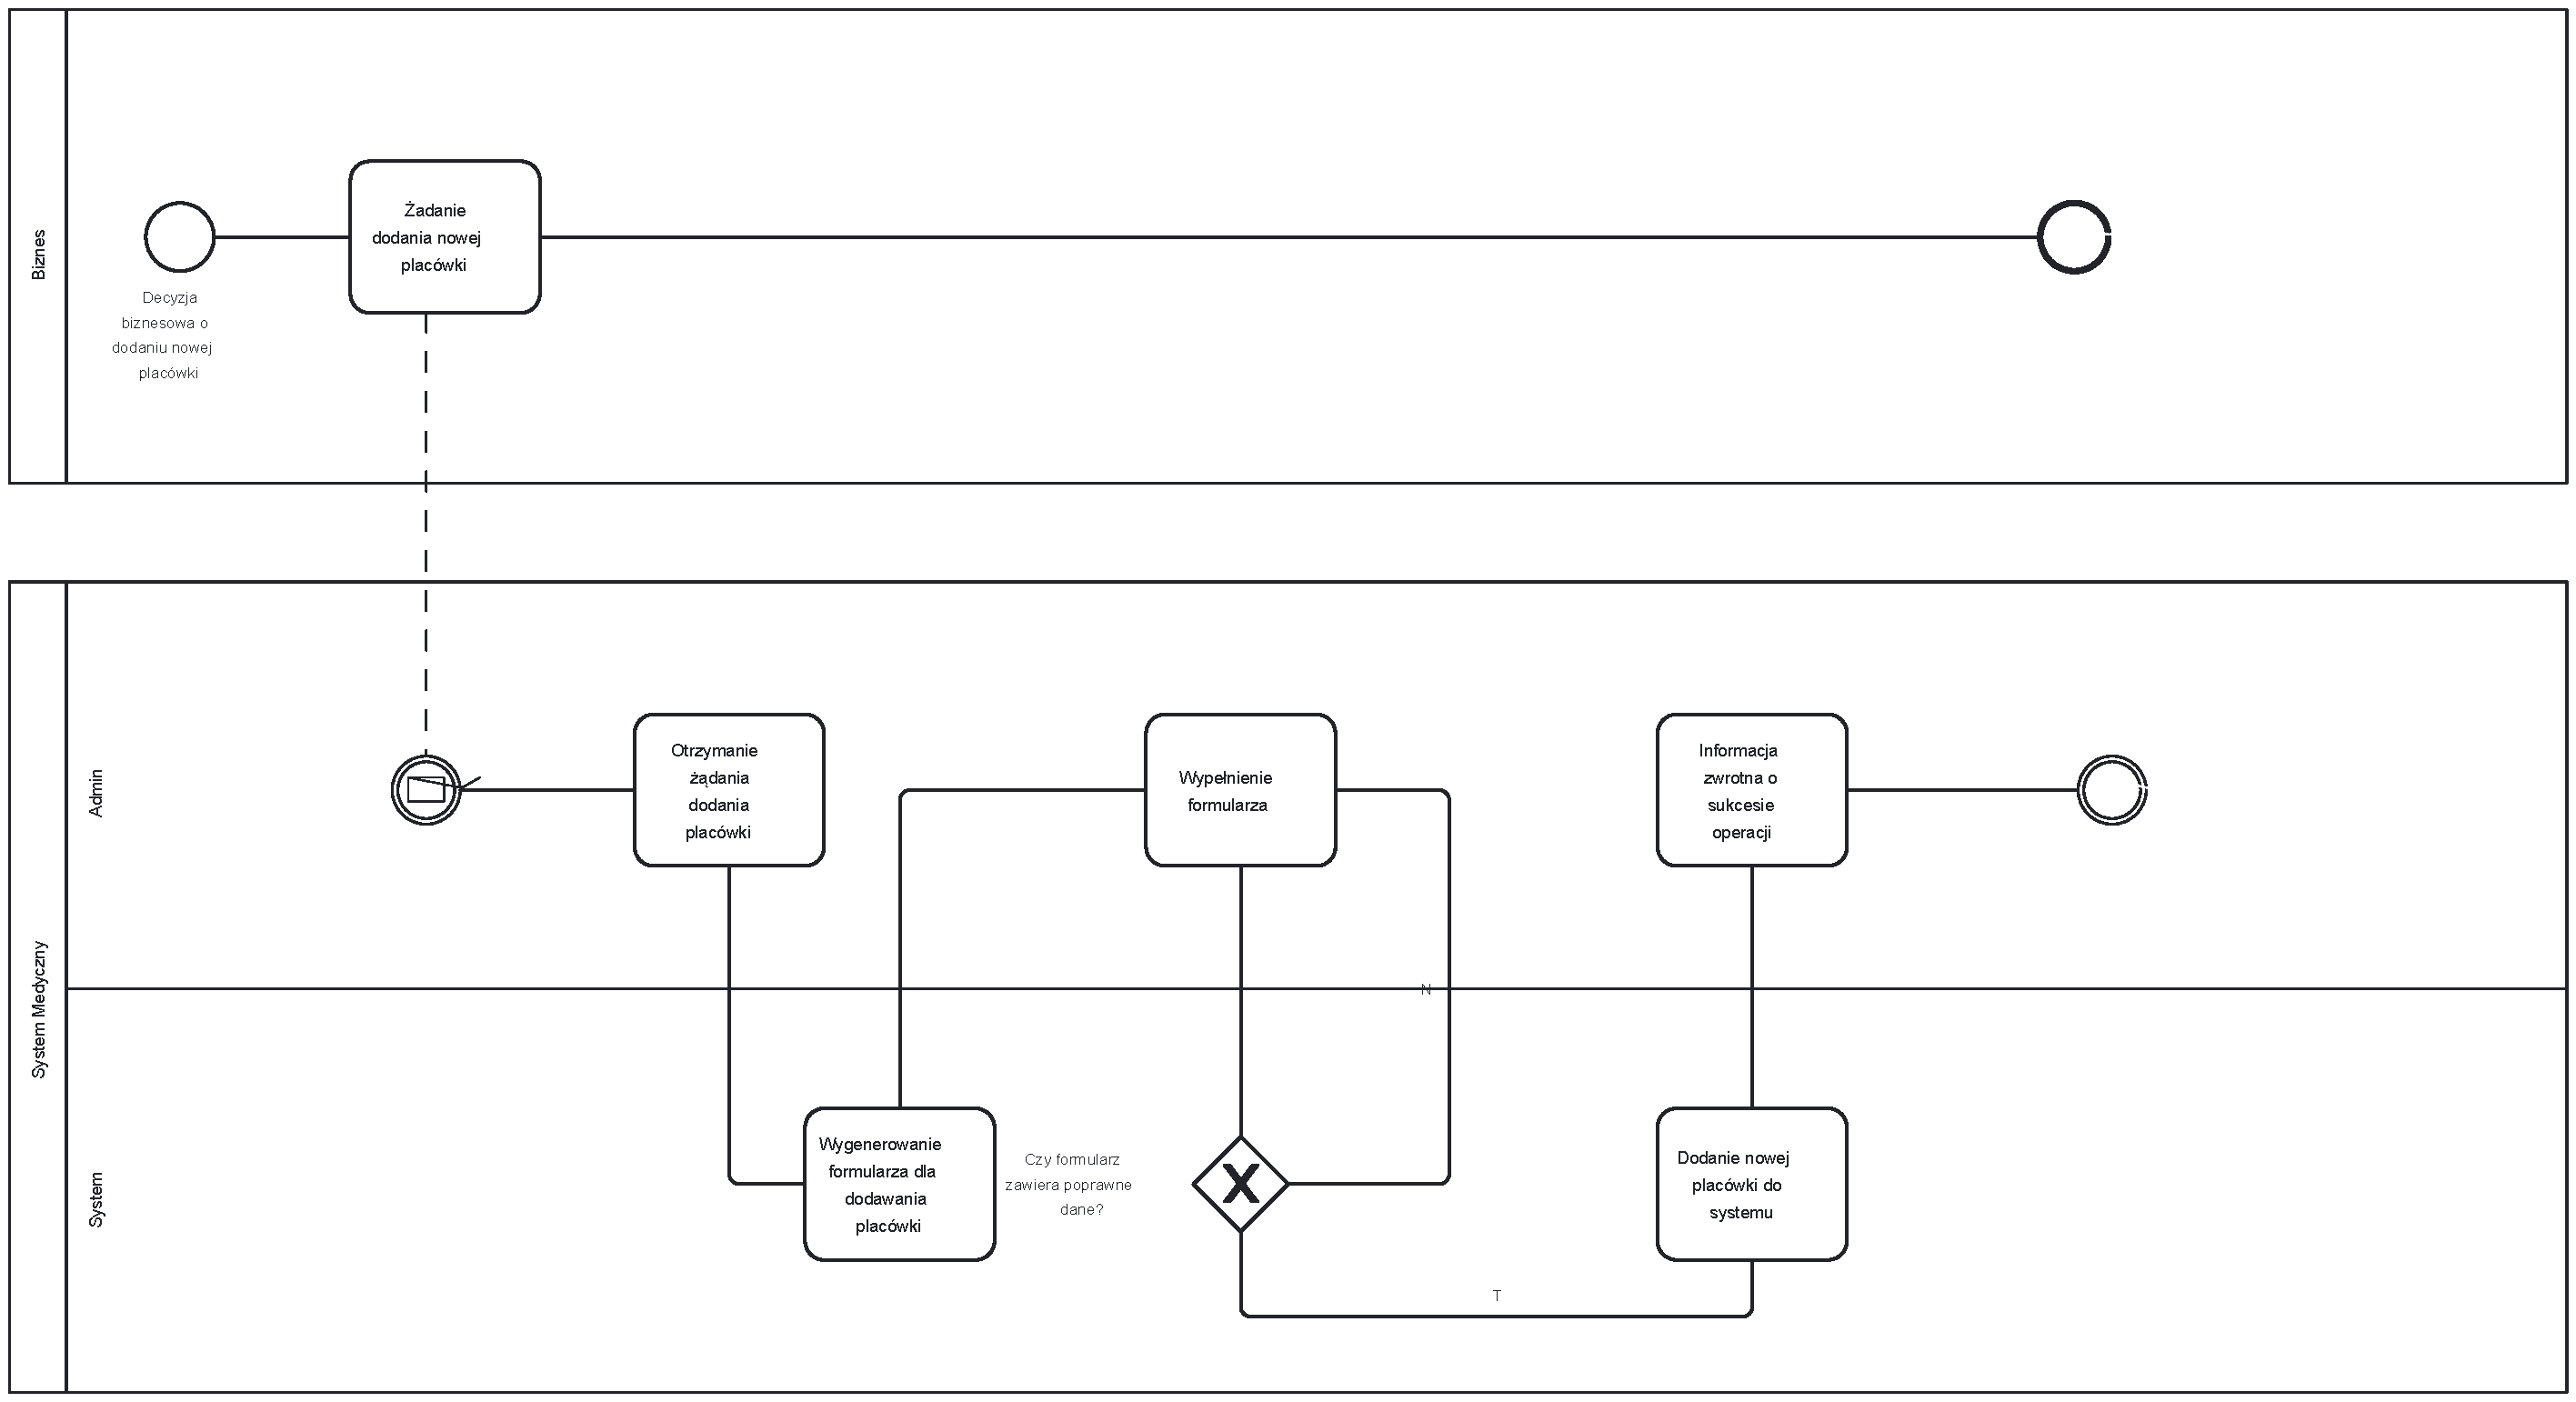
\includegraphics{bpmn/FacilityRegistrationAdmin.pdf}
  }
  \caption{Rejestracja/zarządzanie placówką (administrator)}
\end{figure}

\begin{figure}[H]
  \centering
  \adjustbox{max width=\textwidth}{
    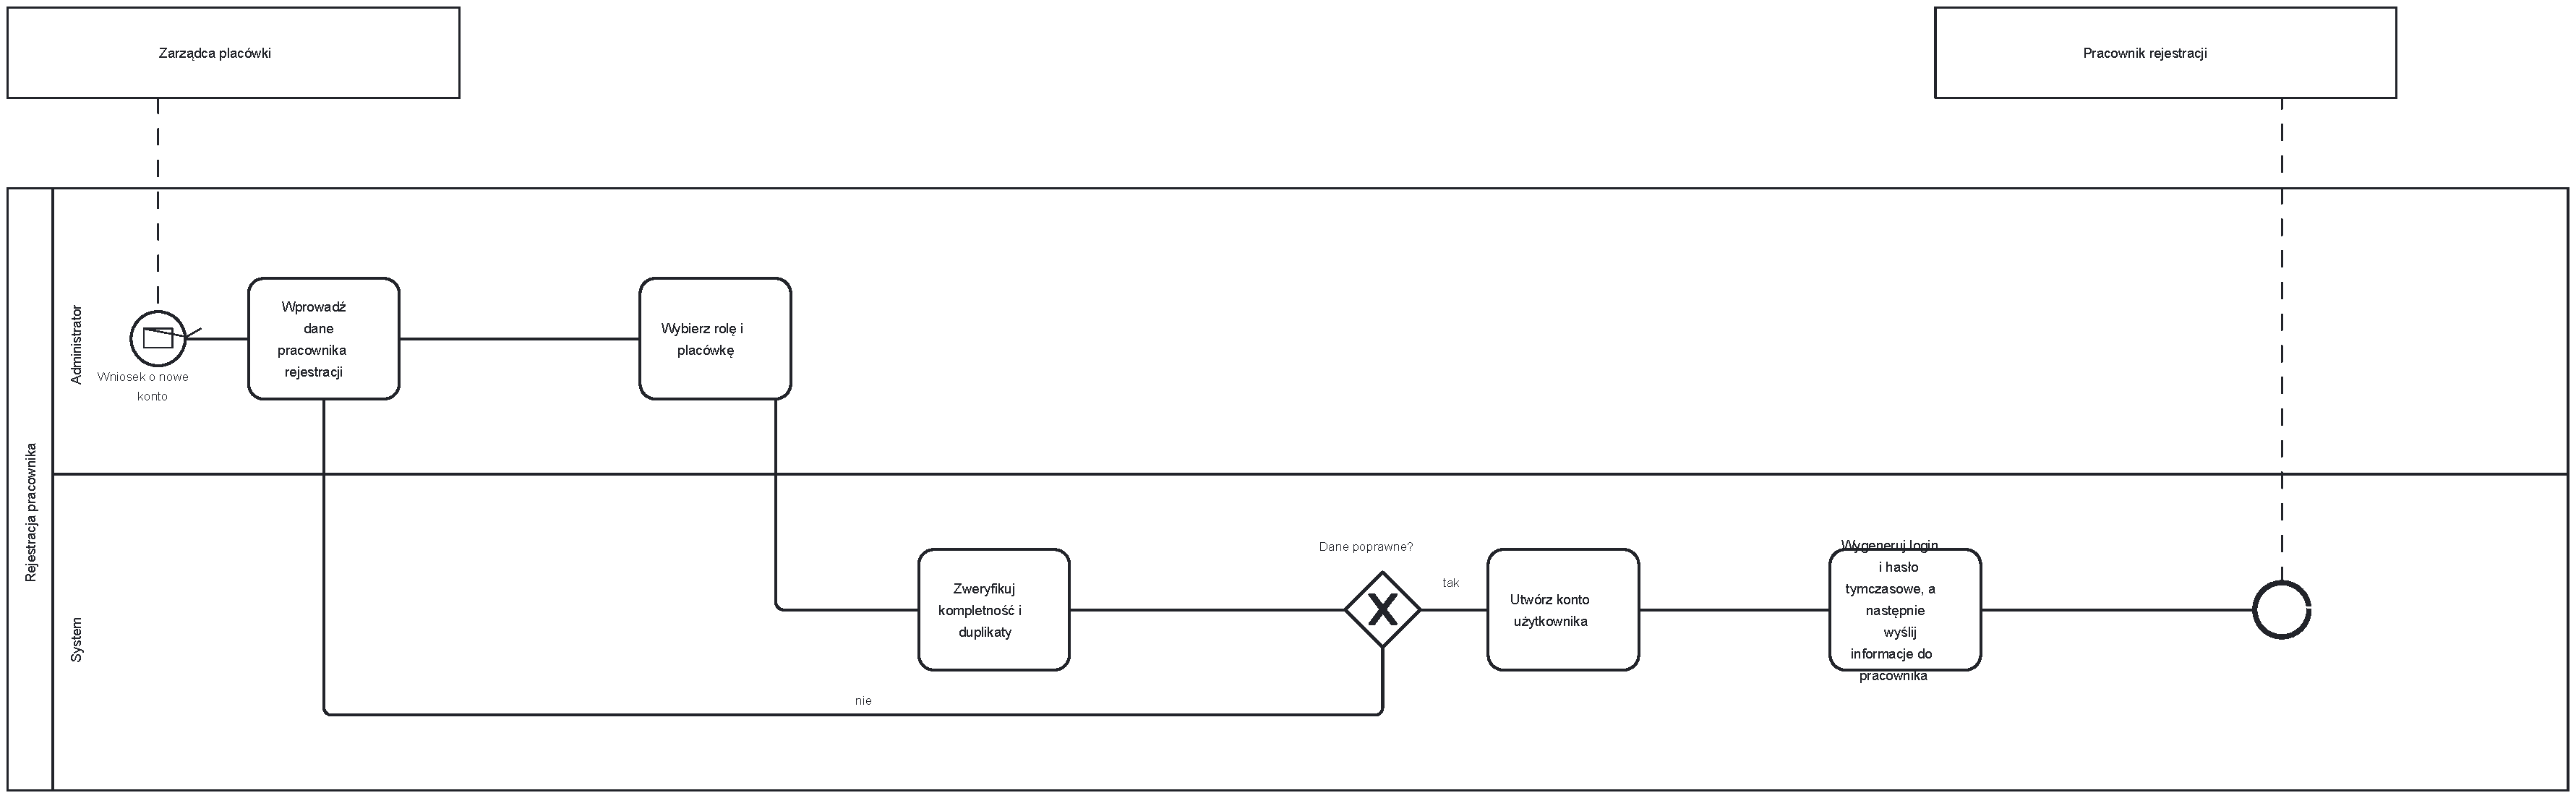
\includegraphics{bpmn/ClerkRegistrationAdmin.pdf}
  }
  \caption{Rejestracja pracownika rejestracji przez administratora}
\end{figure}

\begin{figure}[H]
  \centering
  \adjustbox{max width=\textwidth}{
    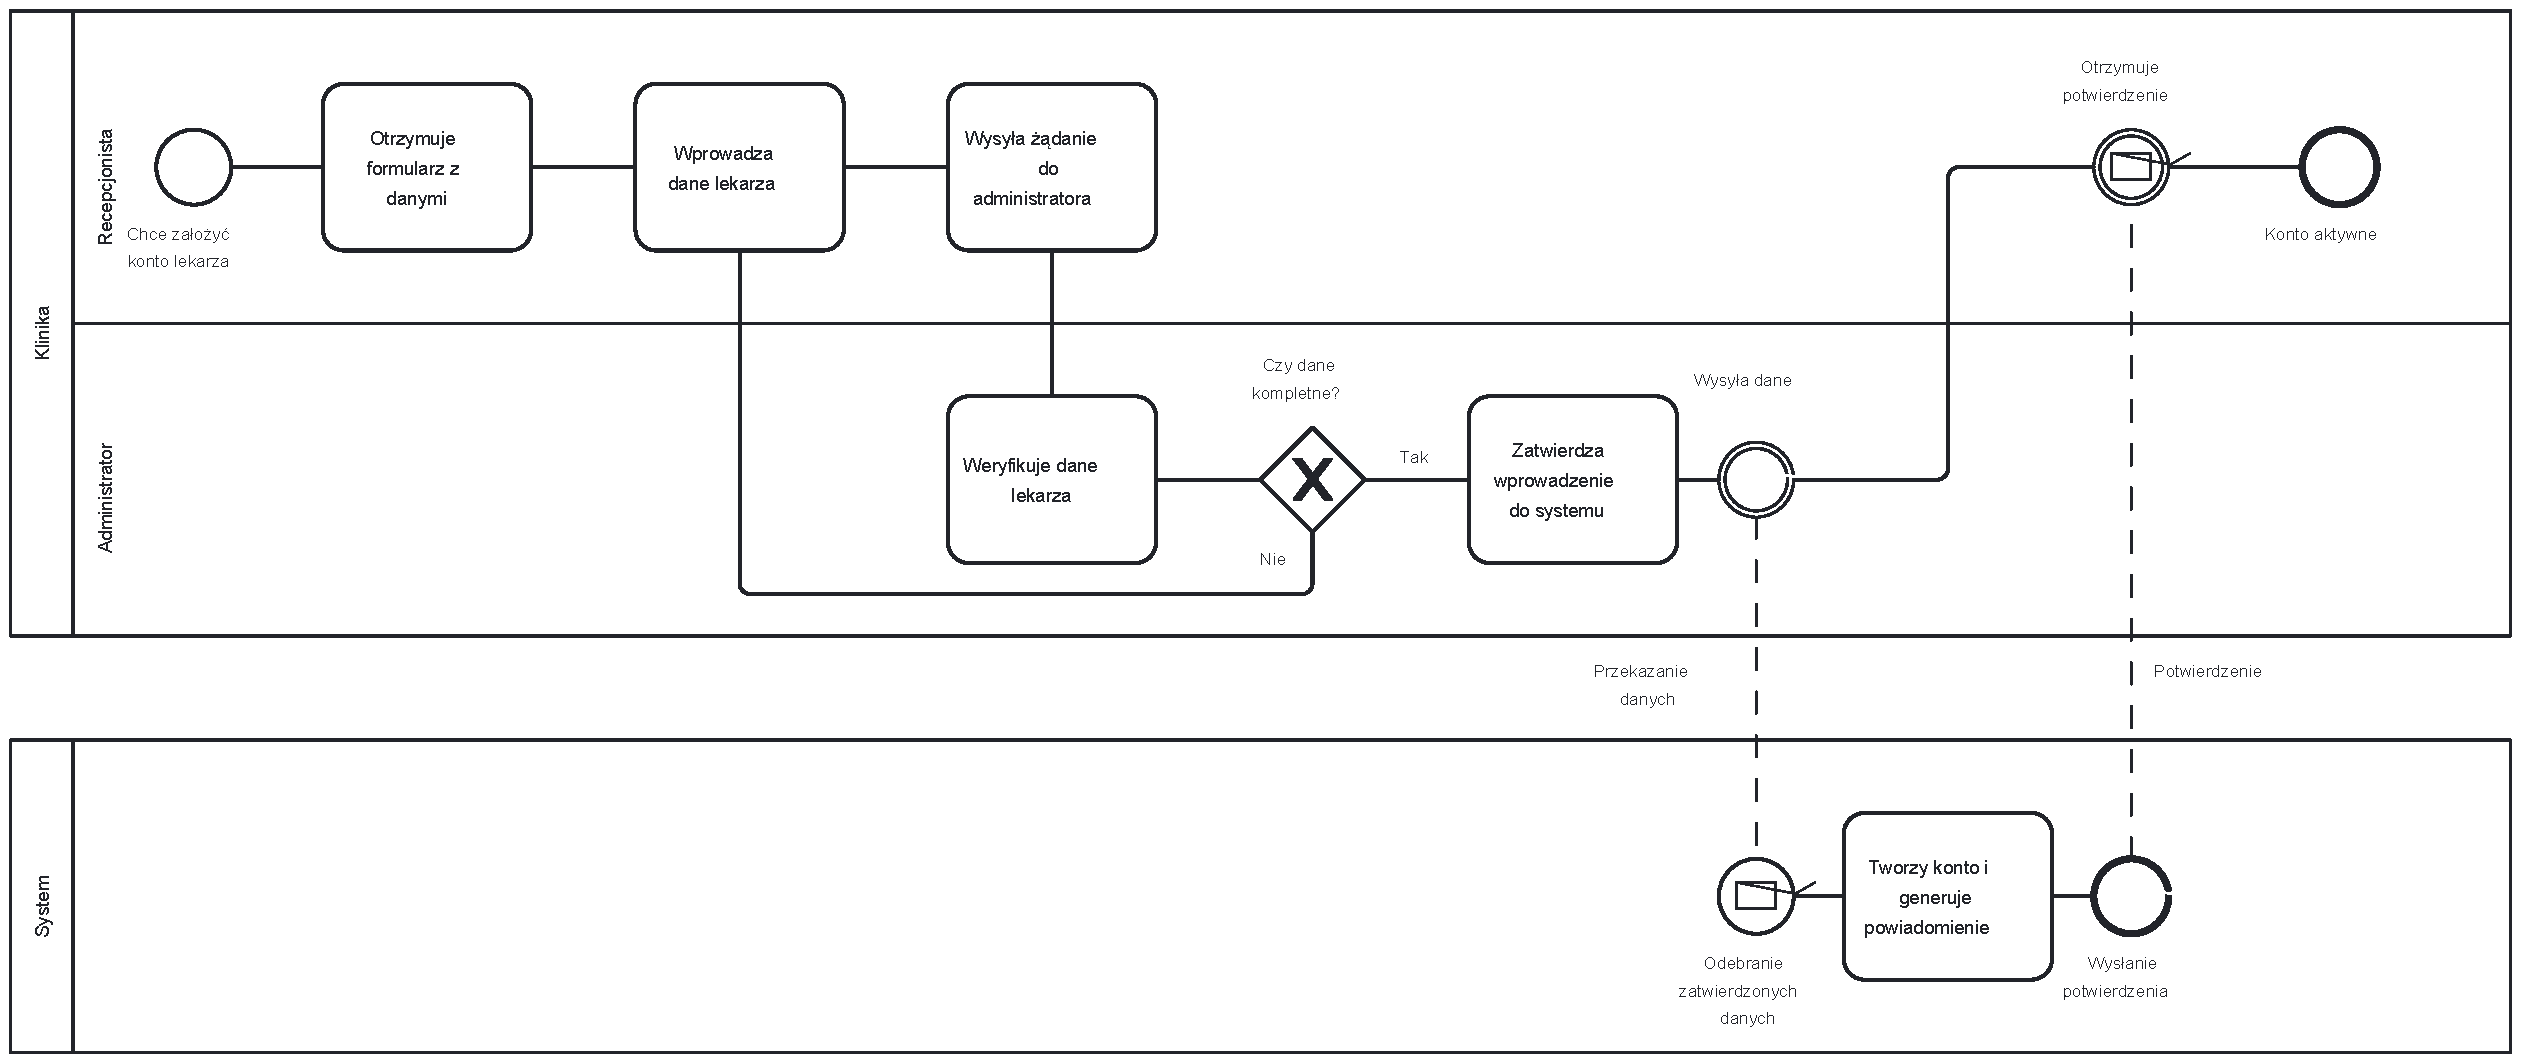
\includegraphics{bpmn/DoctorRegistrationClerk.pdf}
  }
  \caption{Rejestracja lekarza przez pracownika rejestracji}
\end{figure}

\begin{figure}[H]
  \centering
  \adjustbox{max width=\textwidth}{
    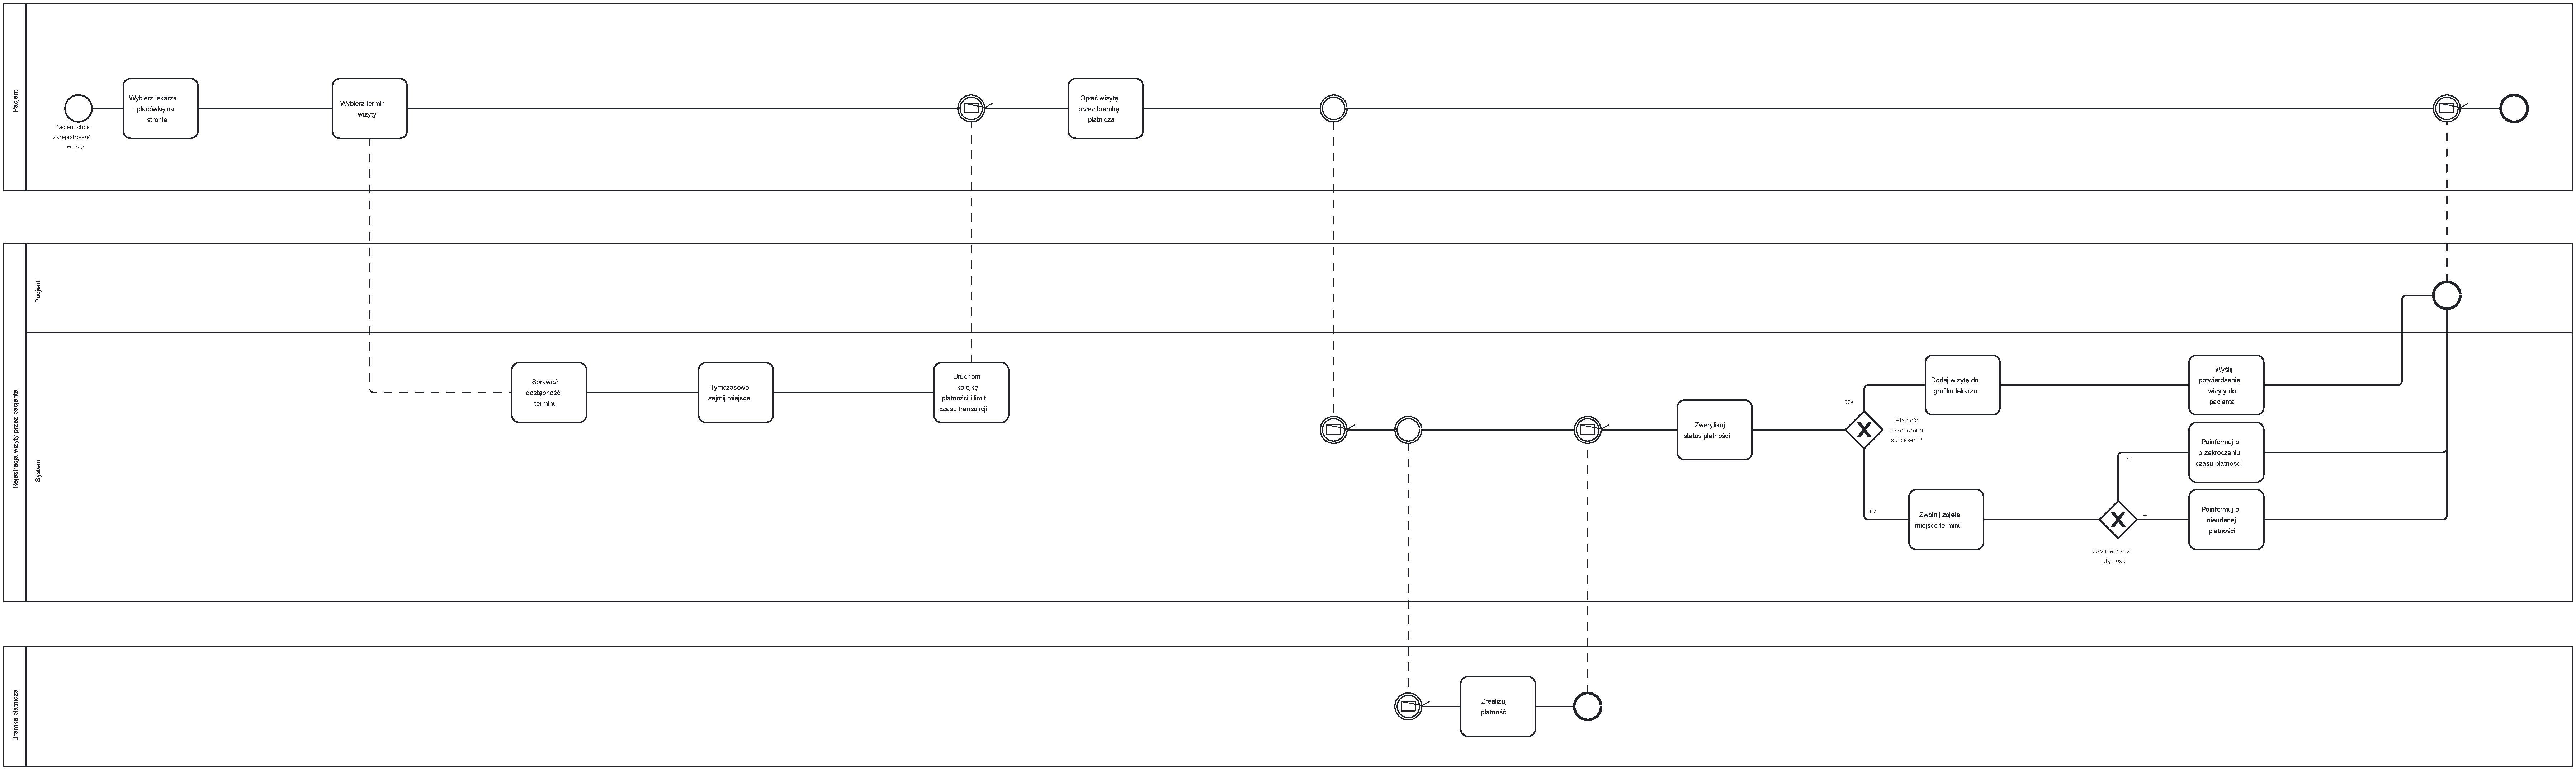
\includegraphics{bpmn/VisitRegistrationPatient.pdf}
  }
  \caption{Rejestracja wizyty przez pacjenta}
\end{figure}

\begin{figure}[H]
  \centering
  \adjustbox{max width=\textwidth}{
    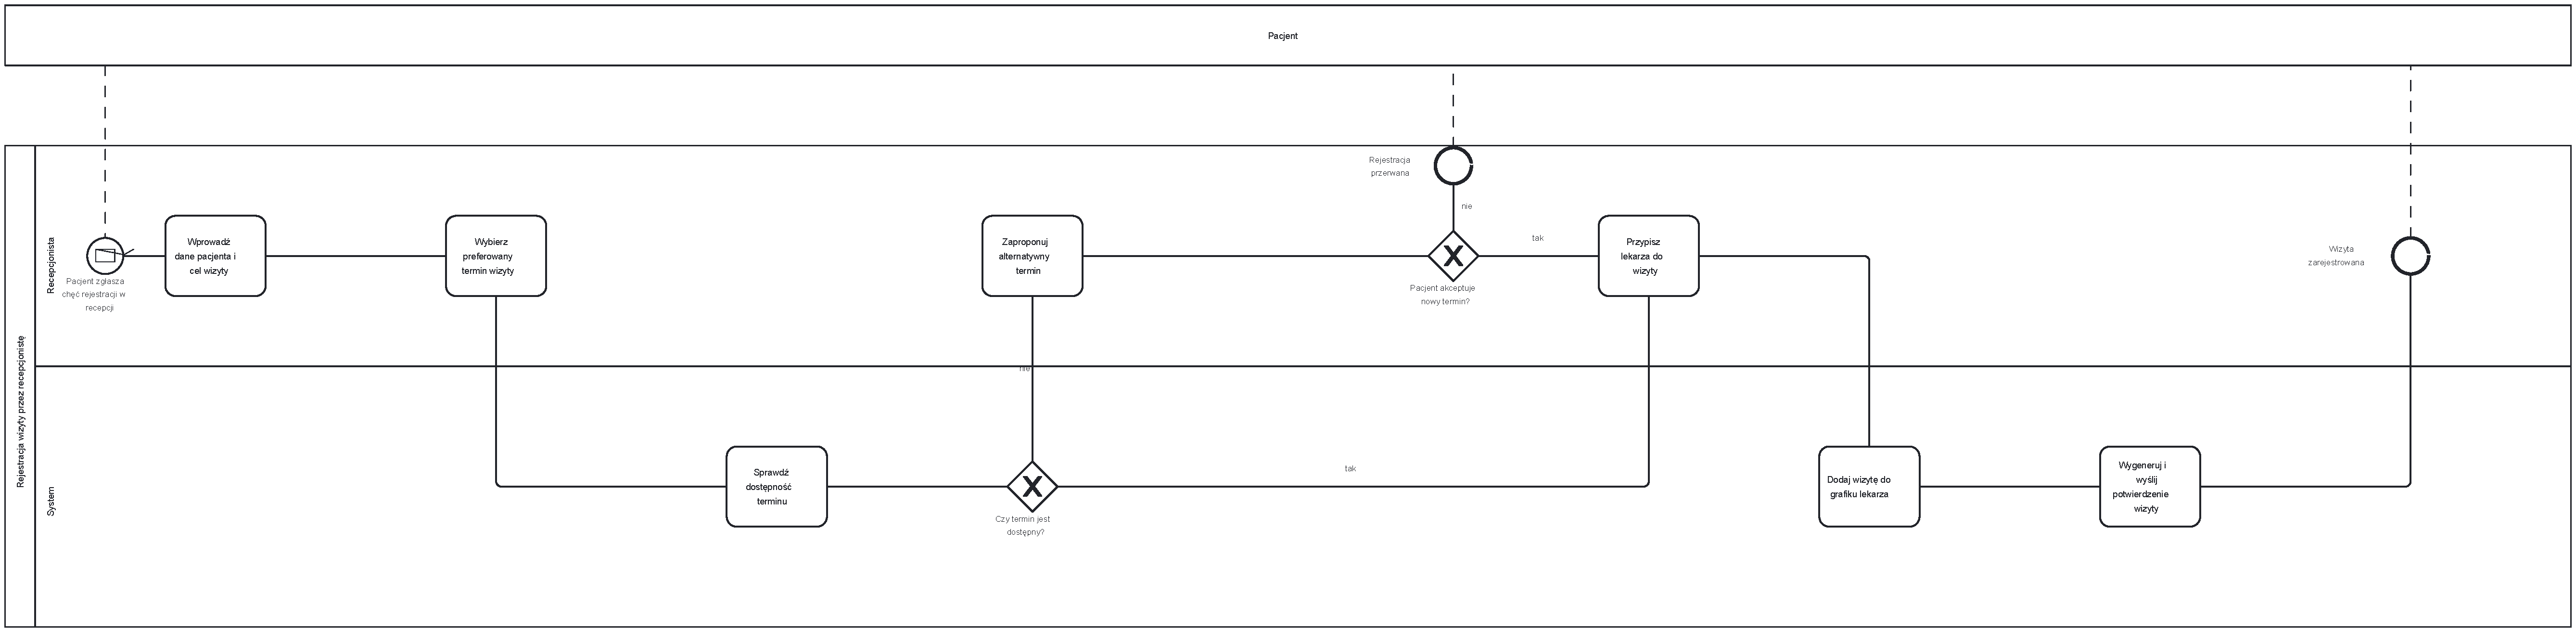
\includegraphics{bpmn/VisitRegistrationClerk.pdf}
  }
  \caption{Rejestracja wizyty przez pracownika rejestracji}
\end{figure}

\begin{figure}[H]
  \centering
  \adjustbox{max width=\textwidth}{
    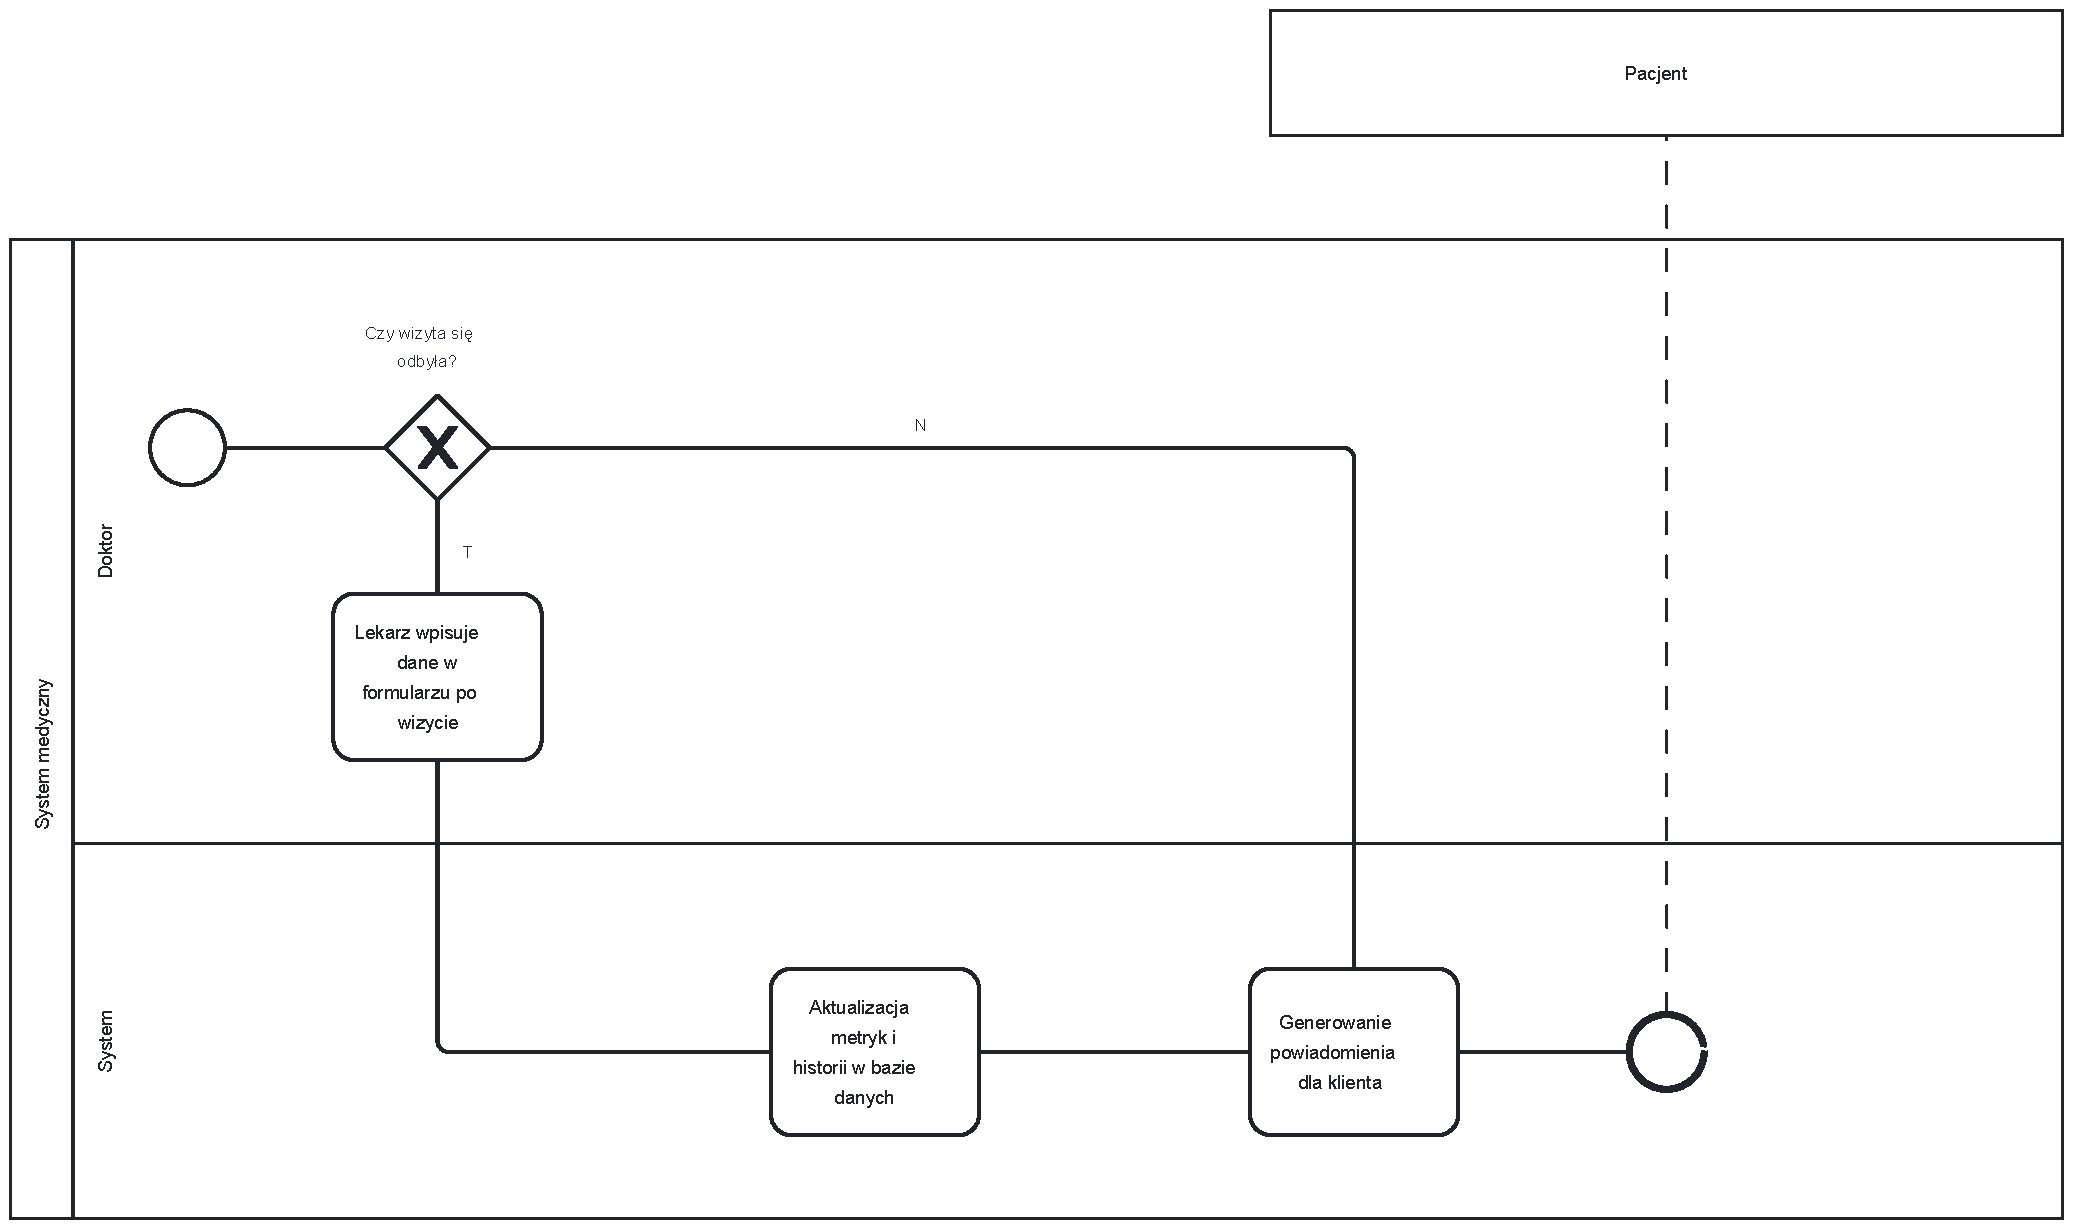
\includegraphics{bpmn/VisitFinishingDoctor.pdf}
  }
  \caption{Zakończenie wizyty przez lekarza}
\end{figure}

\begin{figure}[H]
  \centering
  \adjustbox{max width=\textwidth}{
    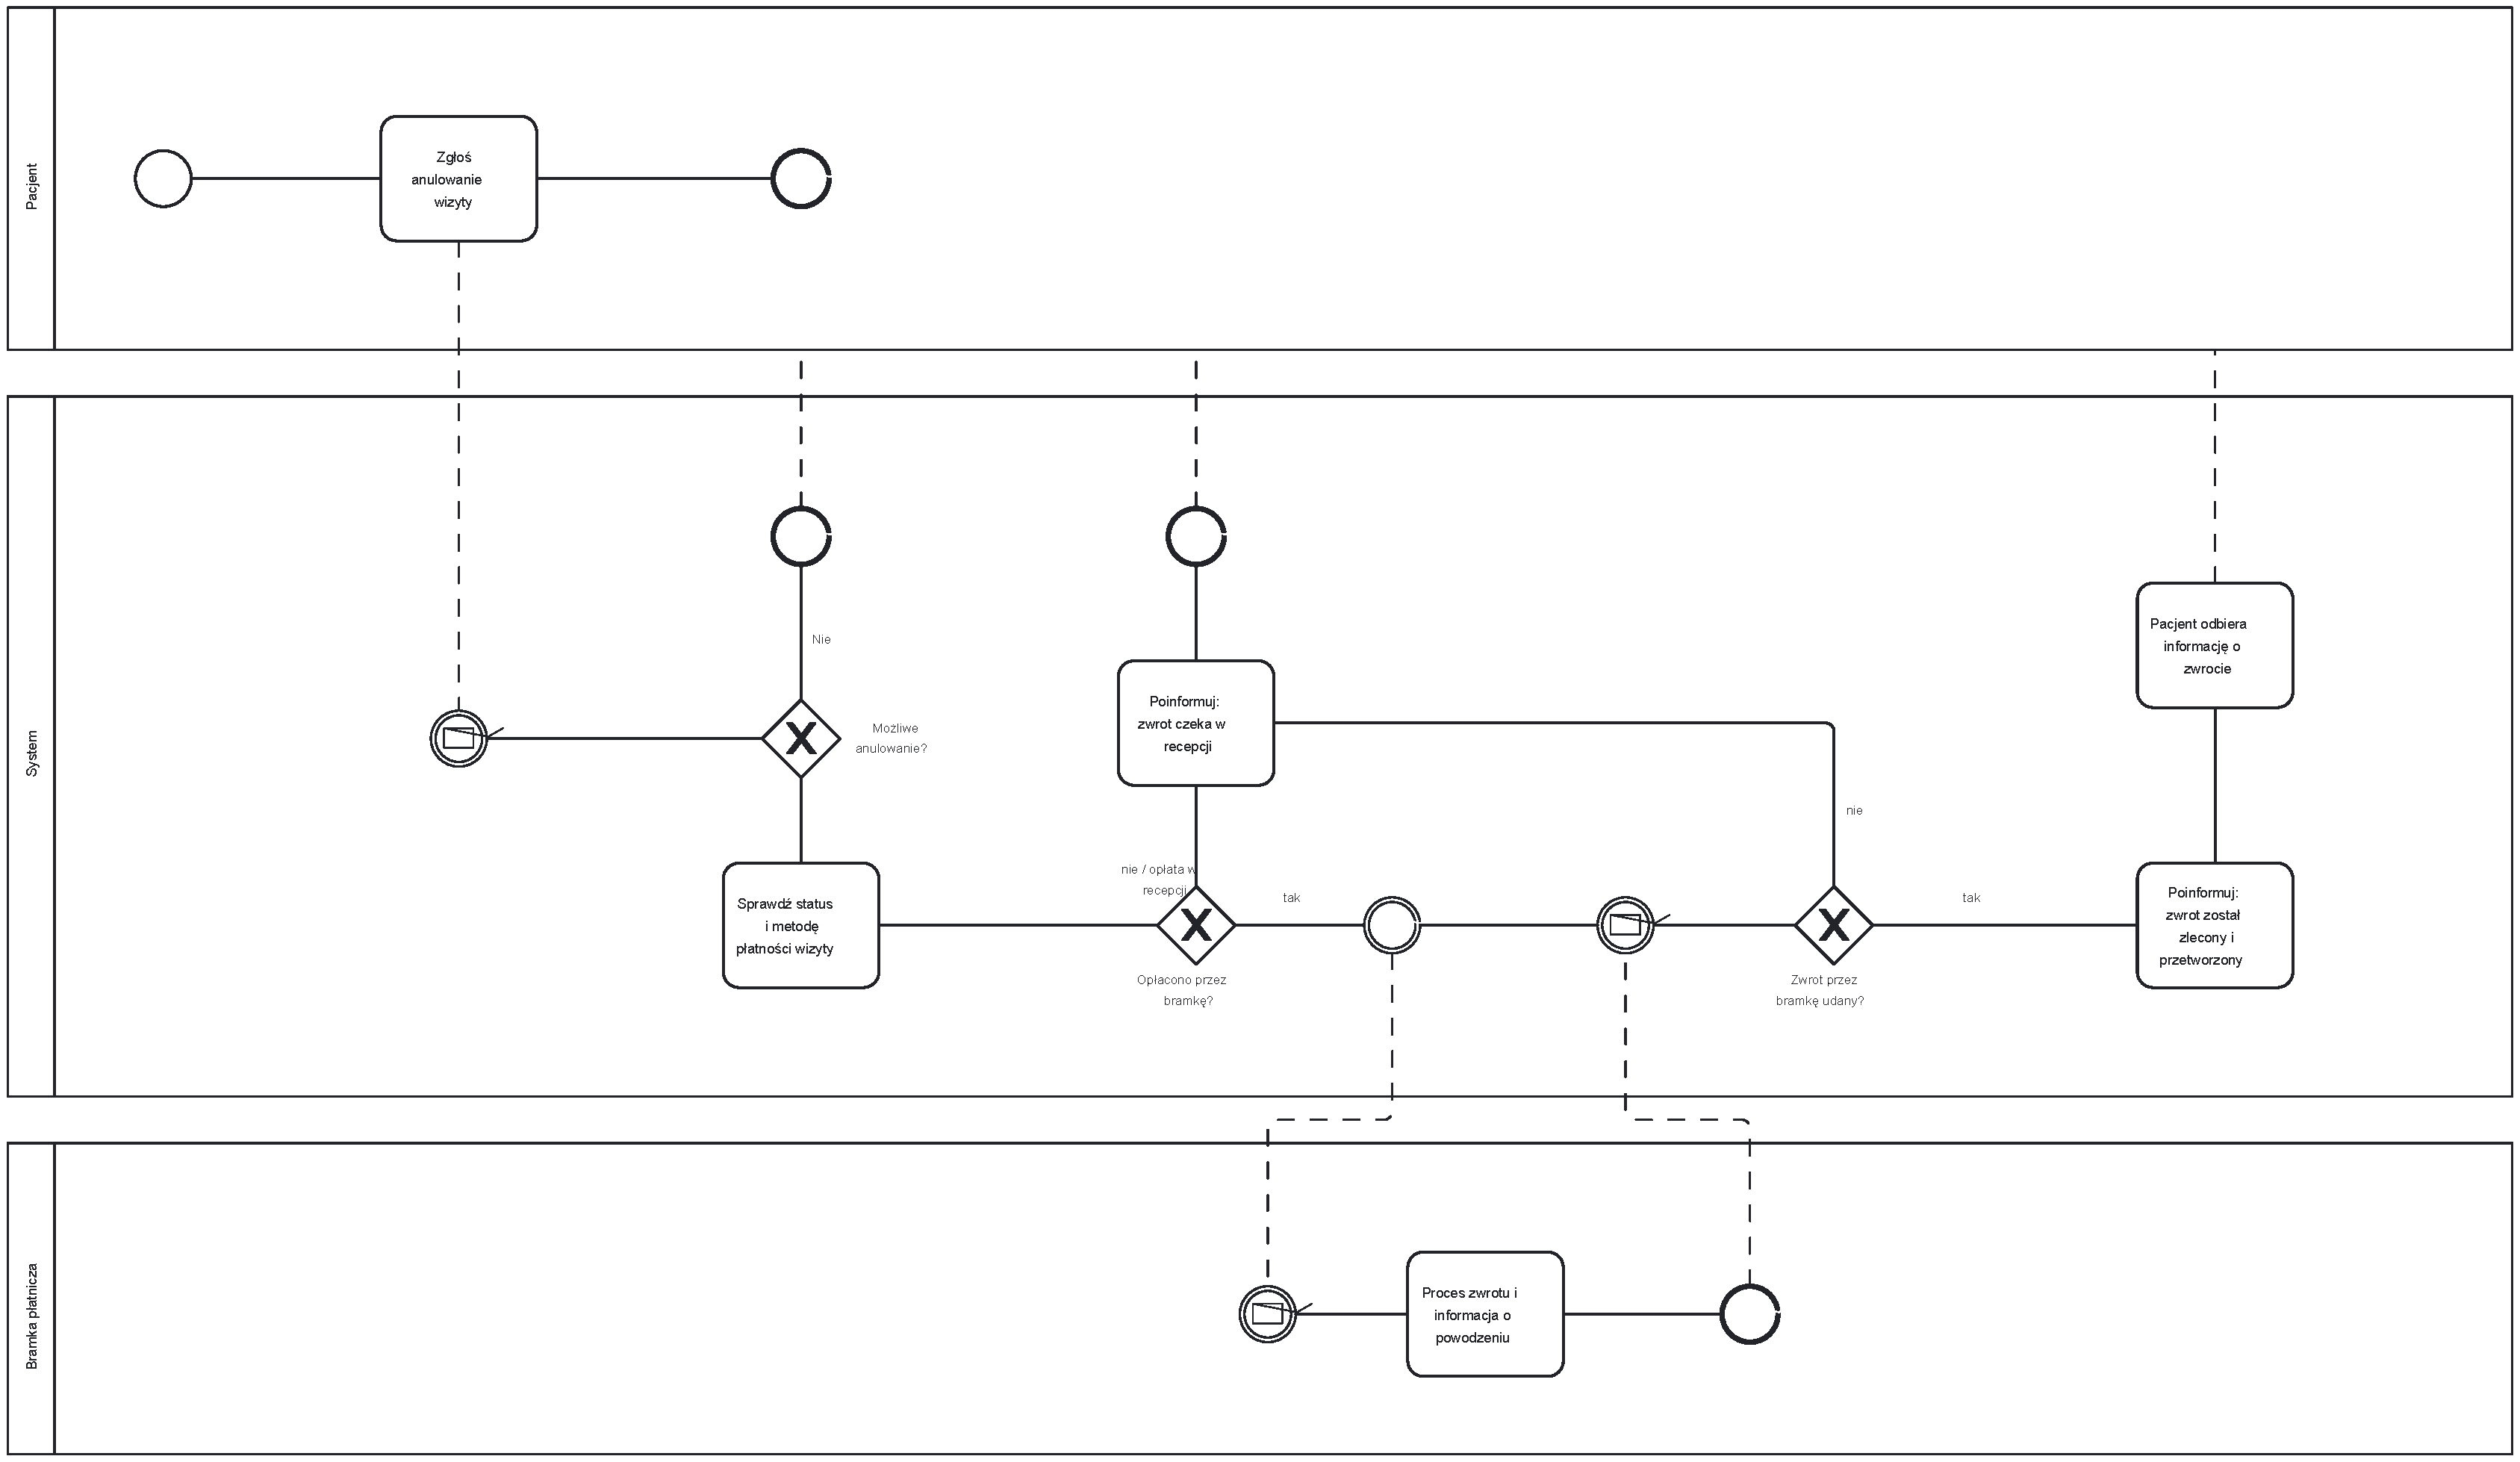
\includegraphics{bpmn/VisitCancelationPatient.pdf}
  }
  \caption{Anulowanie wizyty przez pacjenta}
\end{figure}

\begin{figure}[H]
  \centering
  \adjustbox{max width=\textwidth}{
    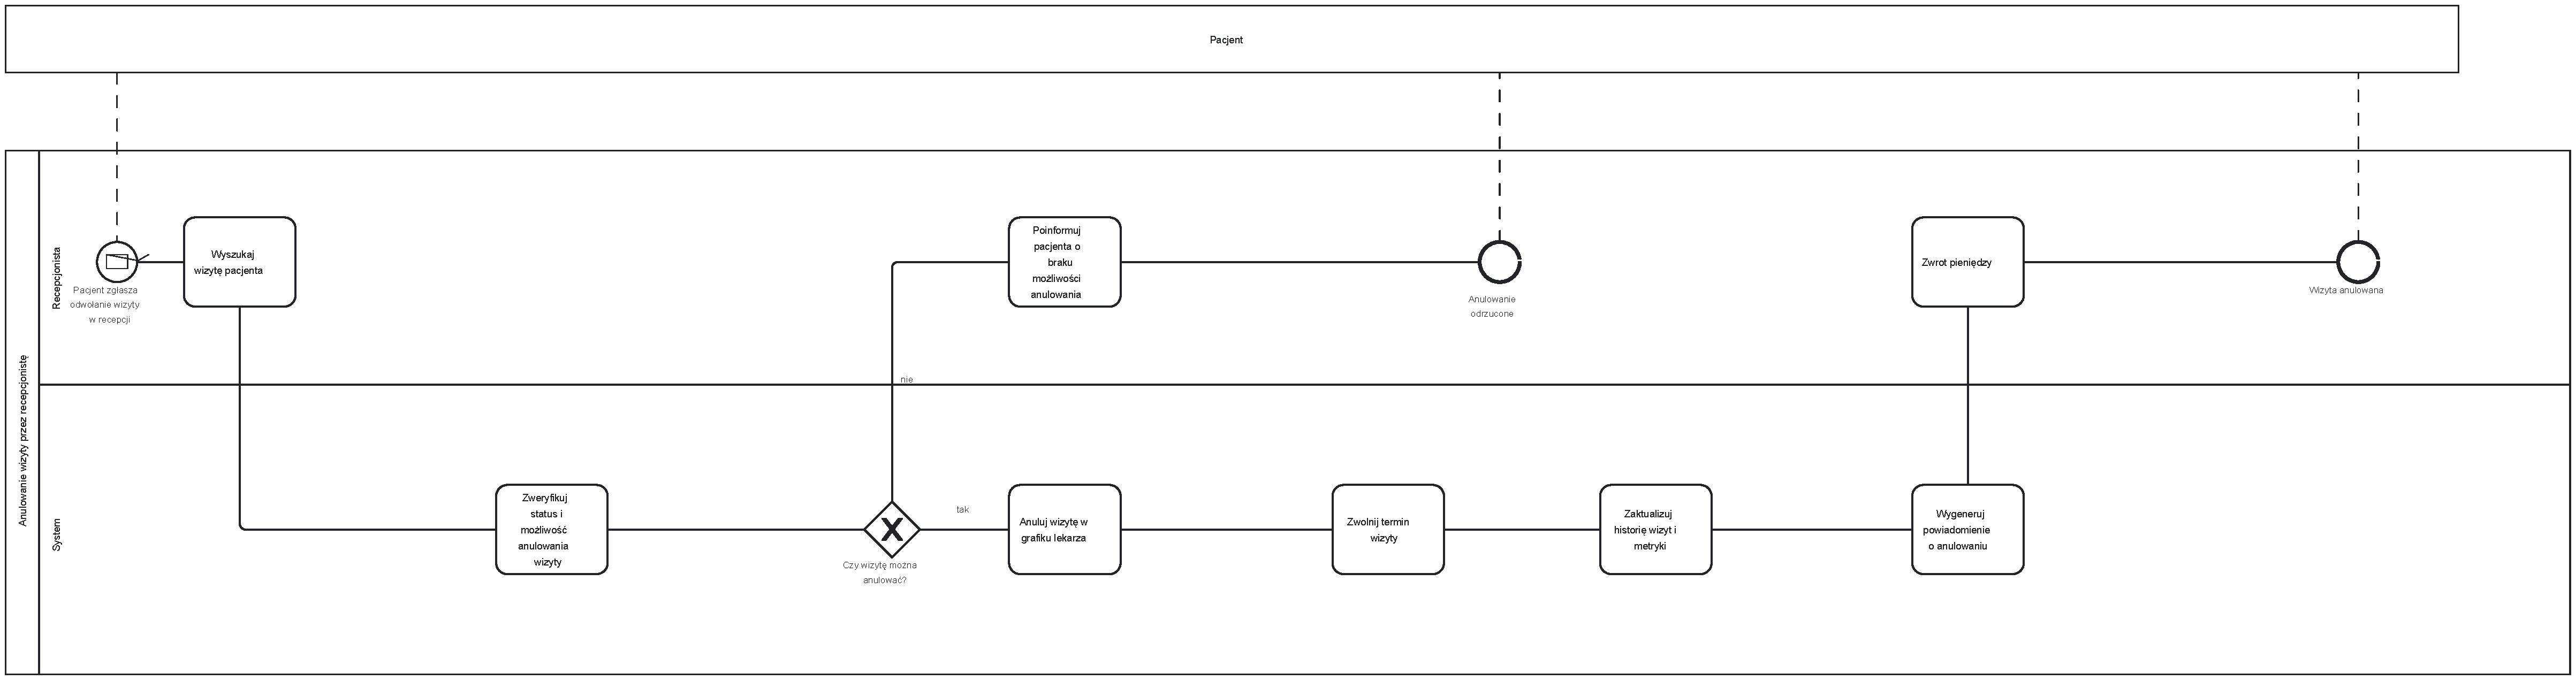
\includegraphics{bpmn/VisitCancelationClerk.pdf}
  }
  \caption{Anulowanie wizyty przez pracownika rejestracji}
\end{figure}

\begin{figure}[H]
  \centering
  \adjustbox{max width=\textwidth}{
    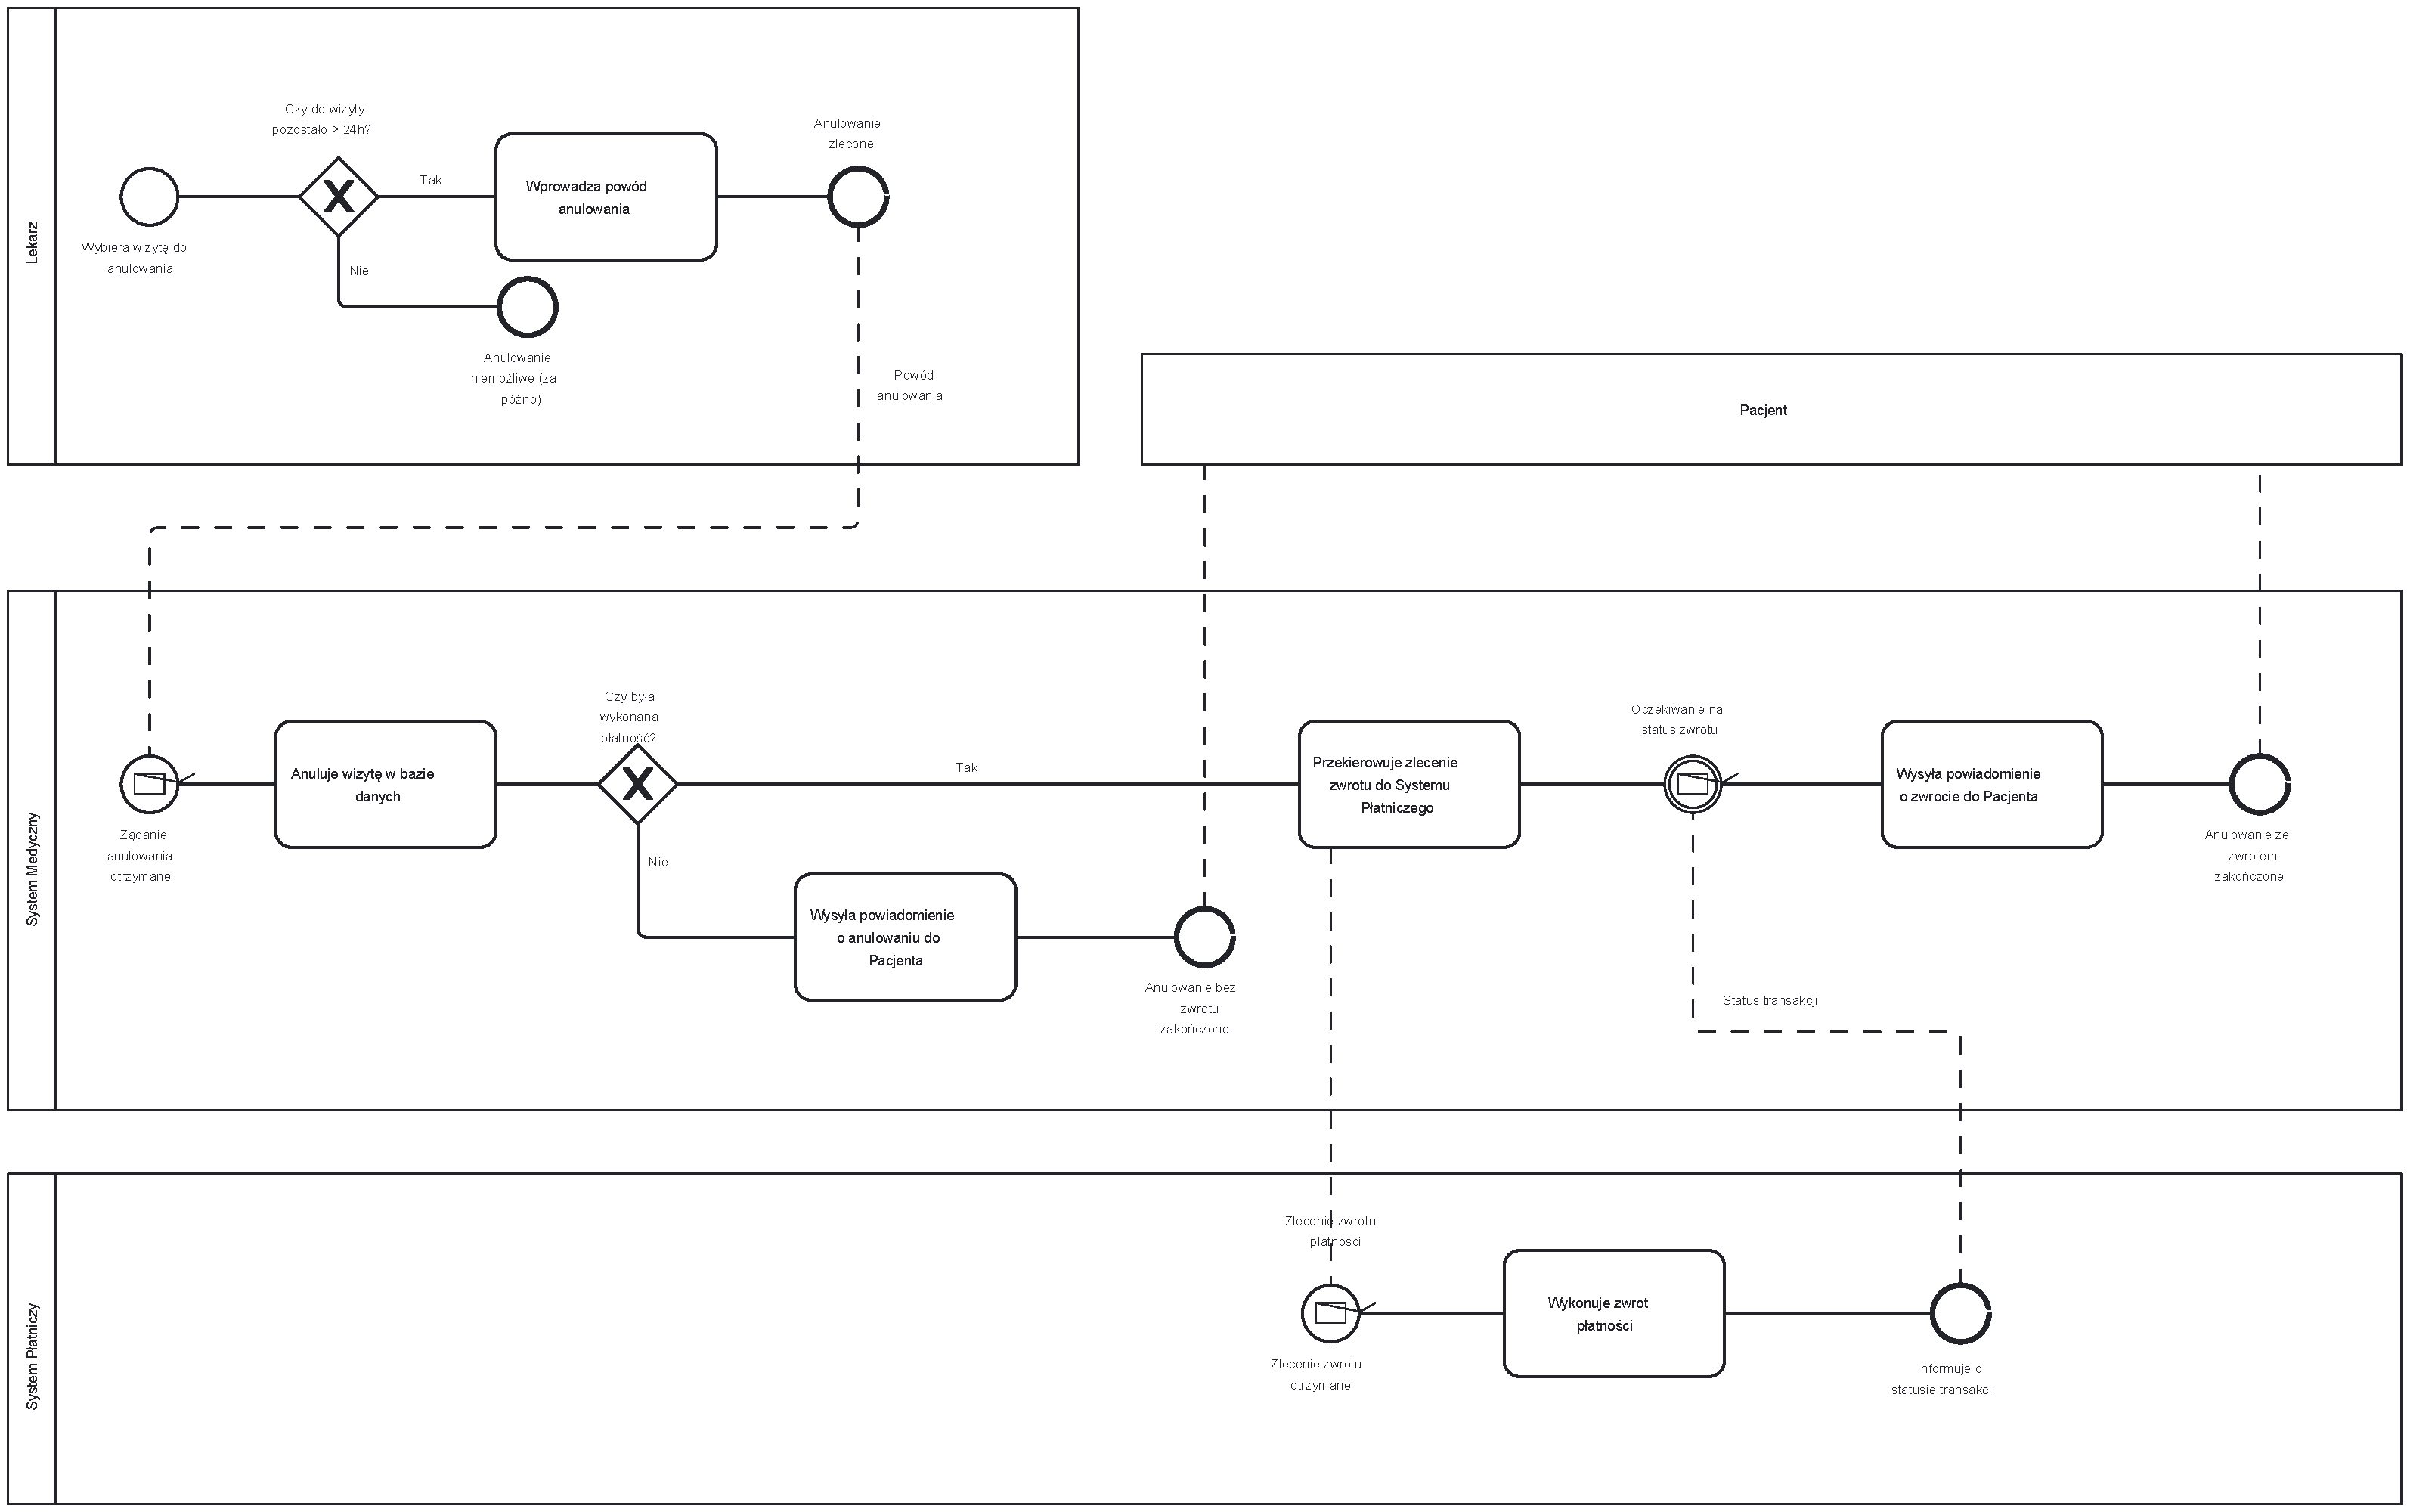
\includegraphics{bpmn/VisitCancelationDoctor.pdf}
  }
  \caption{Anulowanie wizyty przez lekarza}
\end{figure}

\subsection{Proces integracyjny w orkiestracji}
\textit{Przykład: Złożony proces płatności i finalizacji rezerwacji.}\\
W tym modelu występuje centralny zarządca procesu – np. dedykowany \texttt{Order-Orchestrator} wewnątrz \texttt{Payment-Service}.
\begin{enumerate}
    \item Orkiestrator wysyła synchroniczne żądanie do API PayU o utworzenie płatności.
    \item Po otrzymaniu pozytywnego statusu płatności, orkiestrator wysyła bezpośrednie żądanie (komendę) do \texttt{Appointment-Service}: "Zmień status wizyty na OPŁACONA".
    \item Dopiero po potwierdzeniu od \texttt{Appointment-Service}, orkiestrator wysyła komendę do \texttt{Notification-Service}: "Wyślij bilet/potwierdzenie z integracją Google Calendar".
\end{enumerate}
Jeśli krok 2 zawiedzie, orkiestrator uruchamia akcję kompensacyjną (np. zleca zwrot środków w PayU).

\section{Założenia systemowe}
System obejmuje obsługę pacjenta, lekarza i administratora.\\
Architektura: mikroserwisy, komunikacja synchroniczna REST i asynchroniczna RabbitMQ.\\
Integracje zewnętrzne: PayU, Gmail API, Google Calendar API.\\
Kanał użytkownika końcowego: portal WWW.\\
\subsection{Wymagania funkcjonalne}
\begin{itemize}
\item System umożliwia rejestrację konta pacjenta przez formularz WWW z walidacją danych.
\item System umożliwia logowanie użytkowników i zarządzanie sesją.
\item System umożliwia wyszukiwanie lekarzy po specjalizacji, placówce i terminie.
\item System prezentuje listę wolnych terminów dla wybranego lekarza i placówki.
\item System umożliwia rezerwację wybranego terminu wizyty przez pacjenta.
\item System blokuje wybrane okno czasowe na czas realizacji płatności online.
\item System uruchamia limit czasu na płatność i po jego przekroczeniu automatycznie zwalnia termin.
\item System integruje się z PayU w celu utworzenia transakcji płatniczej dla rezerwacji.
\item System odbiera i przetwarza webhooki PayU o zmianie statusu płatności.
\item Po potwierdzeniu płatności system zmienia status wizyty na opłacona.
\item Po niepowodzeniu płatności system anuluje rezerwację i zwalnia termin.
\item Po opłaceniu wizyty system dodaje wizytę do grafiku lekarza.
\item System wysyła potwierdzenie rezerwacji do pacjenta e-mailem.
\item System wysyła przypomnienia o nadchodzącej wizycie.
\item System synchronizuje wydarzenia wizyt z Google Calendar pacjenta i lekarza.
\item Pacjent może anulować własną wizytę zgodnie z regułami biznesowymi.
\item System realizuje zwrot płatności online po anulowaniu wizyty opłaconej przez PayU.
\item Jeśli zwrot online nie powiedzie system oznacza zwrot do odbioru w recepcji i informuje pacjenta.
\item Jeśli płatność była offline jest do zwrotu, system oznacza zwrot do odbioru w recepcji i informuje pacjenta.
\item Lekarz może definiować dostępność i blokować terminy.
\item Lekarz ma podgląd wizyt na dzień i tydzień.
\item Lekarz może dodawać notatki medyczne i zalecenia po wizycie.
\item Pacjent ma dostęp do historii wizyt, dokumentów i rachunków/faktur.
\item Administrator zarządza kontami personelu i pacjentów oraz ich rolami.
\item Administrator zarządza słownikiem usług, cennikami i konfiguracją integracji.
\item Administrator ma dostęp do logów operacyjnych i raportów finansowych.
\item Każdy mikroserwis udostępnia REST API opisane w OpenAPI 3.0.
\item Wejściowe payloady API są walidowane przez JSON Schema, a błędne żądania kończą się 400 Bad Request.
\item System publikuje zdarzenia domenowe do RabbitMQ, w tym appointment.created, appointment.canceled, payment.success, payment.failed.
\item Proces płatności i finalizacji rezerwacji jest obsługiwany przez orchestrator z akcjami kompensacyjnymi przy błędach.
\item System implementuje ślad audytowy w postaci logowania zmiam w bazie i aktorów inicjujących je. 
\end{itemize}

\subsection{Wymagania niefunkcjonalne}
\begin{itemize}
\item Czas odpowiedzi API dla 80 percentyla poniżej 5000 ms dla operacji odczytu.
\item Czas odpowiedzi API dla 80 percentyla poniżej 10000 ms dla operacji zapisu.
\item System obsługuje minimum 100 jednoczesnych użytkowników bez degradacji krytycznych funkcji.
\item Potwierdzenie statusu płatności z webhooka PayU jest przetwarzane do 60 sekund od otrzymania.
\item Kolejki RabbitMQ muszą gwarantować trwałość komunikatów i brak utraty danych przy chwilowej niedostępności usług.
\item Każda operacja krytyczna musi być idempotentna, zwłaszcza webhooki płatności i zmiany statusu wizyty.
\item System musi spełniać wymagania RODO, w tym minimalizację danych i możliwość realizacji praw podmiotu danych.
\item Dane w tranzycie są szyfrowane TLS 1.2 lub nowszym, dane w spoczynku szyfrowane po stronie bazy i magazynu plików.
\item Dostęp do API i paneli administracyjnych jest chroniony mechanizmami uwierzytelniania i autoryzacji ról.
\item Wszystkie akcje administracyjne i medyczne są logowane w audycie z identyfikatorem użytkownika i znacznikiem czasu.
\item Backup bazy danych wykonywany minimum raz na dobę, retencja minimum 30 dni.
\item System musi umożliwiać niezależne skalowanie mikroserwisów.
\item Dokumentacja API w OpenAPI musi być aktualna i publicznie dostępna dla zespołu w Swagger UI.
\item System zapewnia centralne logowanie, metryki i alertowanie dla usług i brokera wiadomości.
\item Interfejs WWW musi być responsywny i wspierać aktualne wersje Chrome, Edge i Firefox.
\item Architektura i kod muszą umożliwiać testy automatyczne API, integracyjne i end-to-end dla procesów krytycznych.
 \end{itemize}

\section{Proponowana infrastruktura w AWS}
\begin{itemize}
    \item \textbf{Amazon EC2 / ECS:} Do hostowania kontenerów z poszczególnymi mikroserwisami. Dla uproszczenia wariantu studenckiego można wykorzystać instancje EC2 za pomocą narzędzia Docker Compose, jednak zalecanym podejściem jest użycie Elastic Container Service (ECS).
    \item \textbf{Amazon RDS:} W pełni zarządzana relacyjna baza danych (PostgreSQL), wykorzystywana jako trwała warstwa przechowywania danych dla mikroserwisów, oferująca automatyczne kopie zapasowe.
    \item \textbf{Amazon S3:} Służy do hostowania statycznych plików aplikacji frontendowej (SPA) oraz do ewentualnego przechowywania plików załączników medycznych (np. skanów wyników badań).
    \item \textbf{Application Load Balancer (ALB):} Do dystrybucji ruchu HTTP/HTTPS przychodzącego z zewnątrz bezpośrednio do API Gateway.
\end{itemize}

\end{document}